\documentclass[10pt]{article}
\usepackage{coqdoc}
\usepackage{graphicx}
\usepackage{float}
\floatstyle{boxed}
\restylefloat{figure}

\title {VLisp: A Formally Verified Lisp\\or\\Explorations in the Formal Verification of McCarthy's Equations}
\author{K. Isom}

\begin{document}
\maketitle

\section{Background}

Alan Kay once described a certain half-page of code in the Lisp 1.5
manual\footnote{http://www.softwarepreservation.org/projects/LISP/book/LISP\%201.5\%20Programmers\%20Manual.pdf}
as 
\begin{quote}
These were ``Maxwell’s Equations of Software!'' This is the whole world of programming in a few lines that I can put my hand over\footnote{http://queue.acm.org/detail.cfm?id=1039523}.
\end{quote}

\begin{figure}[h]
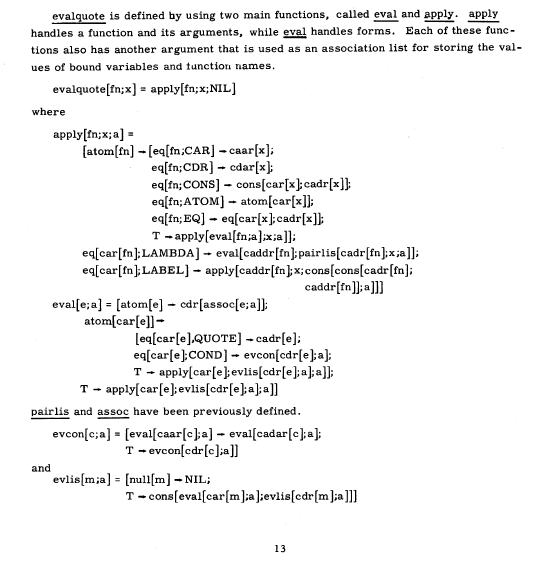
\includegraphics{Lisp_Maxwells_Equations}
\caption{McCarthy's Equations of Software}
\end{figure}

(These equations are described in Figure 1.) If we posit that these
equations are, in fact, an analogue of Maxwell's equations that
capture a description of ``the whole world of programming'' in a
mathematically-precise language, can a formally-verified
implementation be built? What does this implementation tell us about
the world of programming?

Some core questions this might immediately invoke are,

\begin{enumerate}
  \item What is the syntax of a formally-verified Lisp?
  \item What are the semantics of a formally-verified Lisp?
  \item What guarantees can we make about the behaviour of this Lisp?
  \item Working under the assumption that Lisp (in particular, a Lisp
    derived from the equations in Figure 1) can be considered as a
    sort of ``McCarthy's Equations of Software'' (MEoS), what theorems
    can be made regarding its behaviour and properties?
  \item What are the practical, useful implications of these theorems?
\end{enumerate}

While the end goal is to build a formal model of Lisp from McCarthy's
equations, it will be necessary to implement the first chapter of the
Lisp 1.5 manual, ``The Lisp Language''.

\section{The Lisp Language}

Before delving into a software implementation, let us consider Lisp,
the language.

McCarthy splits the language into two formats:

\begin{itemize}

\item \emph{S-expressions} (symbolic expressions) are the notation of
  Lisp programs,

\item \emph{M-epxressions} (meta-expressions) are the notation of the
  source language that specifies how to process S-expressions.

\end{itemize}

Immediately we are presented with the question of representation; that
is, how to separate the quotidian task of rote parsing of input text
from the extraction of the central tents, the core of the language?
What does it mean to be an S-expression? An S-expression consists of
either

\begin{itemize}
  \item an atomic symbol
  \item or composed of a pair of S-expressions
\end{itemize}

Syntactically, an atomic symbol is a string of characters (starting
with a letter); the Lisp 1.5 manual imposes the limitation that the
characters composing an atomic symbol be restricted to numbers and
capital letters. In this paper, we'll follow this form for atomic
symbols (and represent them in fixed width font) to distinguish them
from other symbols. An S-expression is either one of these atomic
symbols, or composed of the form $($sexpr . sexpr$)$.

Examples of S-expressions:

\begin{itemize}
  \item \verb|ATOM|
  \item $($\verb|A| . \verb|B|$)$
  \item $($\verb|A| . $($\verb|B| . \verb|C|$))$
\end{itemize}

\input{Lisp}
\end{document}